\documentclass{standalone}
\usepackage{tikz}
\usetikzlibrary{calc,intersections}
\usepackage{animate}
\begin{document}
%==================
\def\sfa{100}
\begin{animateinline}[controls,autoplay,palindrome,loop]{2}
\multiframe{\sfa}{i=0+1}{
%\foreach \i in {0,1,...,\sfa}{
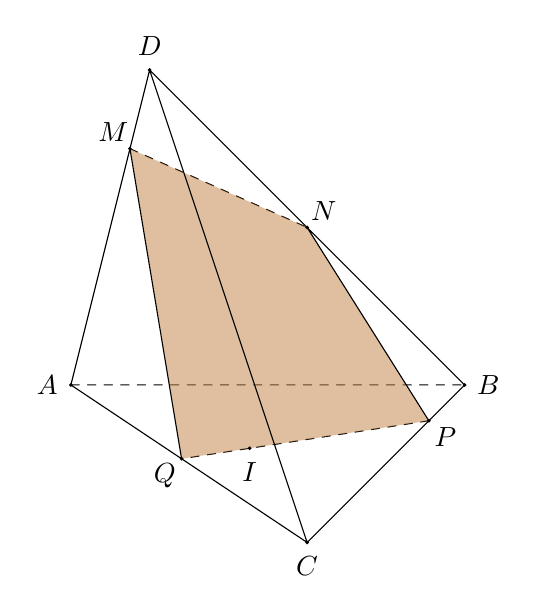
\begin{tikzpicture}[join=round,cap=round,]
\pgfmathsetmacro\ka{abs(rand)}
\pgfmathsetmacro\kb{abs(rand)}
\pgfmathsetmacro\kc{abs(rand)}
\path
(0,0) coordinate (A)
(5,0) coordinate (B)
(3,-2) coordinate (C)
(1,4) coordinate (D)
(barycentric cs:D=3,A=1) coordinate (M)
(barycentric cs:D=1,B=1) coordinate (N)
(barycentric cs:A=\ka,B=\kb,C=\kc) coordinate (I)
(intersection of M--N and A--B) coordinate (K)
(intersection of I--K and A--C) coordinate (Q)
(intersection of I--K and B--C) coordinate (P)
;
\pgfresetboundingbox
\draw[dashed] (M)--(N) (A)--(B) (P)--(Q);
\fill[brown,opacity=.5] (M)--(N)--(P)--(Q);
\draw 
(D)--(A)--(C)--(B)--cycle
(D)--(C) (N)--(P) (Q)--(M)
;
\foreach \x/\g in {D/90,A/180,B/0,C/-90,M/135,N/45,P/-45,Q/-135,I/-90}\fill (\x) circle (.025)+(\g:.3)node{$\x$};
\end{tikzpicture}
}
\end{animateinline}
\end{document}